\chapter{Man of Mystery}

\begin{wrapfigure}{O}{\figwidth}
	\begin{center}
		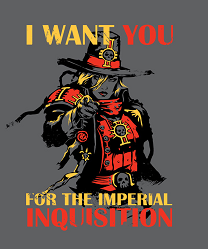
\includegraphics[width=\figwidth]{pics/9/1.png}
	\end{center}
\end{wrapfigure}
This is the ongoing tale of a bunch of guardsmen who got drafted into the Inquisition after their regiment was reduced to a mere 37 men by a combination of Orks, Heretics, more Orks, Tyranids and, of course, their own leadership. 
Currently they work for an Inquisitor that is the 40k equivalent of Professor Oak, he provides teams and missions to Interrogators who need to get some leadership experience before becoming full Inquisitors.

\greentext{>Most previous chapters can be found here:}

http://suptg.thisisnotatrueending.com/archive.html?searchall=all+guardsmen

\begin{wrapfigure}{O}{\figwidth}
	\begin{center}
		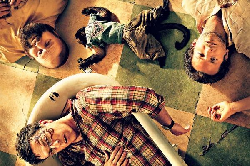
\includegraphics[width=\figwidth]{pics/9/2.png}
	\end{center}
\end{wrapfigure}
Sarge's head hurts. 
He is lying in a pile of rubble, one of his eyes isn't working, he can't feel his left arm, and the only thing he can hear over the ringing in his ears is muffled coughing coming from some debris on the other side of the dimly lit room. 
While he watches, a hand claws its way out of the wreckage and seizes the edge of a table, seconds later it is followed by the scrawny arm, scrawnier chest, and helmeted head of Nubby. 
Sarge tries to croak a warning as the trooper overbalances and falls against the wall, but he's too late, the entire room is filled with blinding light and screams.

Cursing loudly and moving with incredible speed, Sarge lifts the table off his arm, staggers to his feet, and switches the lights back off. 
All around the room figures are sitting up and swearing at Nubby between pained groans. 
A half empty bottle sails out of a small furniture fortress and just barely misses the trooper. 
In a croaking voice Sarge asks if anyone remembers where they are, why an eyepatch and tricorn hat have been glued to his head, and who the trooper duct-taped to the ceiling is.

Twitch is frantically searching his fort for several personal items that seem to be missing, outside there's an ominous click as Sarge finds one of them. 
In the middle of the frantic scramble to defuse the mine a tall man wearing a bathrobe and holding a cup of recaff walks in.

The man takes in the wrecked room and its mostly sleeping occupants then casually picks his way towards the troopers. 
He steps around the spot where Sarge is trying not to move and makes his way to Twitch's fortress, where he retrieves a suit-jacket and a few pieces of feminine clothing that were used in the construction. 
As the man heads back out he reminds everyone that their shuttle leaves in two hours.

Up on the ceiling the squad's new technical expert, Tink, wakes up and immediately slams his head into the metal plating.

\greentext{>The All Guardsmen Party And The Interplanetary Man of Mystery}


\begin{wrapfigure}{O}{\figwidth}
	\begin{center}
		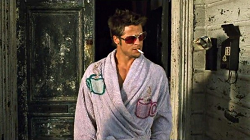
\includegraphics[width=\figwidth]{pics/9/3.png}
	\end{center}
\end{wrapfigure}
So no shit, there we were, five hungover guardsmen in a shuttle conference room, getting briefed on a desertion problem so massive that a literal army of Commissars couldn't stop it. 
At least that's what we thought the briefing was about, it had been written by an Inquisitor with an accent so thick that he was nearly impossible to understand and he'd felt the need to include that accent in his writing. 
This problem was compounded by the fact that the bathrobe-wearing man reading it obviously didn't really give a damn and would often skip whole sections or pause to inject snarky comments.

The man in the bathrobe was our new Interrogator. 
We'd been hanging out in our section of Oak's ship when this guy burst in, dodged Twitch's reaction shot, and threw a briefcase into Sarge's lap. 
Then, without so much as pausing to introduce himself, he told us we had an hour to get the the party started before the girls arrived and left again. 
The briefcase was full of money and marked 'Evidence'.

We didn't over-think the situation, Nubby grabbed a few other guardsmen and went to get supplies, Sarge formed an impromptu cleaning detail, and the rest of the squad went to see who else was up for a good time. 
Things were already getting pretty lively when the mystery man returned over a dozen sororitas and half of the all-female assassination team from Deck G in tow. 
Just saying that we were surprised really doesn't do the situation justice, if it weren't for the large supply of liquid courage most of the guardsmen present would have fled in terror.

It was one hell of a party, shame none of us could really remember it afterwards.

\begin{wrapfigure}{O}{\figwidth}
	\begin{center}
		
\includegraphics[width=\figwidth]{pics/9/4.png}
	\end{center}
\end{wrapfigure}
Right as things had been really getting started the mystery man came over to where we were sitting and pulled Tink, the rather infamous regimental techie, out of the crowd. 
He briefly introduced himself as Bane Johns, said he was our new Interrogator, and told us to go enjoy ourselves. 
When Sarge asked about the mission the Interrogator just said he'd brief us and introduce the rest of the team later, they were busy doing 'boring stuff'. 
After that he wandered off and got a high stakes poker game started with the leftover money from the briefcase, leaving us with the rather confused techie.

After that things were a bit of a blur, but a few incidents stood out. 
Nubby spectacularly lost the poker game and got a black eye after making a rather impertinent remark to Doc's hospitaller lady-friend. 
Tink was thoroughly rejected by Hannah the cog-girl, then got into a heated argument with Twitch over whether an autogun could turn someone into an Ork. 
That ended with Doc taking away most of Twitch's weapons and Tink somehow wound up taped to the ceiling. 
Doc disappeared after the incident and didn't show up until the morning, when he wandered in smelling of flowery anti-septic and helped cut Tink down. 
No one could remember what Sarge did during the party, why he was dressed like a Rogue Trader, or whose idea the glue and permanent marker was.

We all remembered the Interrogator though, he was everywhere during the party. 
He drank more than anyone could really believe, won the poker game, and left with a sister hanging on each arm after laying out two guardsmen during a rather spectacular brawl. 
Then come morning he was up and moving without showing a single sign of discomfort. 
It was almost enough to make you hate him.

\begin{wrapfigure}{O}{\figwidth}
	\begin{center}
		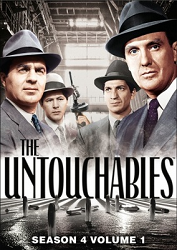
\includegraphics[width=\figwidth]{pics/9/5.png}
	\end{center}
\end{wrapfigure}
The half-assed briefing came to a crashing halt when the rest of our team came in and demanded to know who we were and why we were on their shuttle. 
In retrospect it's easy to see why they didn't recognize us as the team's muscle, none of us looked very professional. 
Twitch and Nubby were obviously hungover, Doc was asleep across a row of chairs, Tink was still half covered with tape, and it was going to take some serious solvents to get the hat and eyepatch off Sarge. 
As for the Interrogator, most folks don't imagine a man lounging around in a bathrobe when they hear the phase "senior Inquisitorial agent".

With one exception the rest of the team consisted of the fifth worst type of people you find in the Inquisition, bureaucrats. 
Coming in right between insane zealots and raging paranoids, they were the sort of extremely serious and tedious individuals that don't derive any actual satisfaction from their life or see why you should either. 
They'd all been some sort of special Arbites team or something, but two of them were just adepts with shock-mauls and the other two were the most tedious arbitrators in existence. 
To a man they were unpleasant to be around, it was easy to see why the Interrogator hadn't invited them to the party, and their fifth was even worse.

He was the absolute worst type of Inquisitorial teammate, a psyker. 
Not a nice sane psyker either, he was a mutterer and radiated a sort of depressing aura. 
His mere presence was so mind-numbing that it was had to be either the result or cause of his teammates' personalities.

The Interrogator got them all calmed before anyone drew a firearm or the psyker exploded, then made a few introductions and ditched us. 
He tossed the briefing documents to one of the adepts and just wandered off, obviously he had better things to do than sit around planning the mission. 
After an hour or so of tedious discussion we all decided he had the right idea and followed suit, no one seemed to notice when we left.

\begin{wrapfigure}{O}{\figwidth}
	\begin{center}
		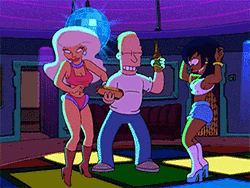
\includegraphics[width=\figwidth]{pics/9/6.png}
	\end{center}
\end{wrapfigure}
That set the tone for the rest of the trip. 
None of us had any desire to spend more time around the gray brigade than absolutely necessary and that included the Interrogator. 
He didn't exclude them from briefings or anything like that, instead he just dumped the whole pile of data provided by the Inquisitors on the bureaucrats and told them to 'handle it'. 
They didn't object to his treatment and we certainly didn't want to get stuck with all the tedious mission planning, but this behavior stuck is as slightly odd. 
As far as we could tell the Interrogator wasn't doing anything to prepare for the near impossible task in front of us, instead he seemed focused on enjoying himself as much as possible during the voyage.

The man seemed to have some sort of superpower, somehow he could get a party started any time, any place, at a moment's notice. 
Every time we saw him he was either telling an amusing story, running a poker game, or had a beautiful woman on his arm. 
It was damned impressive, especially given that we were on a navy vessel, not a cruise ship. 
The only problem was that we couldn't keep up.

At first we tagged along behind Bane, he was the best source of entertainment on the ship, but the man was perfectly capable of drinking until three every single night. 
After a week we gave up and just stood back and watched, it was mind boggling and in Doc's professional opinion the man wasn't human. 


We couldn't hold it against the Interrogator though, he was just a natural born party animal and did his best to make sure we enjoyed ourselves when we joined him, but it was vaguely worrying that he was the one in charge of the mission.

\begin{wrapfigure}{O}{\figwidth}
	\begin{center}
		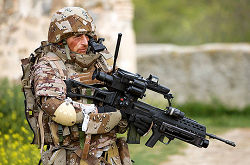
\includegraphics[width=\figwidth]{pics/9/7.png}
	\end{center}
\end{wrapfigure}
While the Interrogator partied and the boring people did boring things, we settled into our own routine and brought Tink properly into the squad.

Tink got his name because 'Fix' would have been confusing on the battlefield and he had the poor taste to complain that Tink was a sissy name when someone called him by it. 
Back in the regiment he had been one of grease monkeys who hung around the motor pool and armory. 
He wasn't an enginseer and got rather snippy if someone called him one, he was just a helper who had picked up far more knowledge than the average tech-priest would want him to have. 
This made him a lot more useful if you wanted to get something fixed without also receiving a lecture on machine spirits and maintenance rituals.

Tink was a solid trooper who pulled his weight despite being rather scrawny and hopeless when it came to close range combat. 
He could fix just about any technical problem a guardsman could have and was the only plasma-trooper we knew that still had all his original fingers and no skin grafts. 
That said Tink wasn't exactly popular with the rest of the regiment; 
the problem was that, not too fine a point on it, he was weird. 
The man had some serious issues with tech-priests, couldn't keep his mouth shut, was nearly as bad as Nubby when it came to respecting personal property, and while he liked to say he had an 'affinity' for technology, the rest of us just called it a fetish.

Prior to joining us he'd been part of a team that was, as far as we knew, still alive and pulling guard duty at some research facility. 
When Doc and Sarge tried to get more info about why he wasn't still with them, all they got was some dark muttering about "hidebound reactionary dinosaurs standing in the way of true science" and "sexual harassment". 
No one felt the need to press further.

\begin{wrapfigure}{O}{\figwidth}
	\begin{center}
		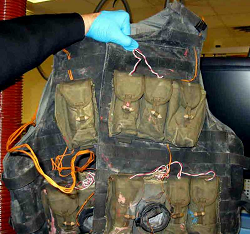
\includegraphics[width=\figwidth]{pics/9/8.png}
	\end{center}
\end{wrapfigure}
Aside from the Interrogator's parties and the occasional meeting with the arbites, we kept to ourselves during the trip. 
Which isn't to say that we just lazed around, from the sound of things we were heading into a combat zone and that's not a safe place for someone who's not prepared for a fight. 
None of us were keen on wasting time reviewing data and making intricate plans with the bureaucrats, instead we focussed on getting our kit and ourselves into top condition.

Sarge led drills, Nubby procured a few extra supplies, and Tink gave almost all of our gear a complete workover. 
Twitch wouldn't let anyone touch his stuff and, after Tink got a look at the modifications Twitch had made, he didn't want to even be in the same room as the demolitions trooper's gear. 
Finally Doc who was rather enthusiastic about his teaching skills after last mission, decided to get together a few group exercises with the rest of the team.

At first everyone assured him that they were perfectly competent and had better things to do, but after enough wheedling everyone agreed just to shut him up. 
The whole team formed up in a half full cargobay and Doc handed out las weapons with training packs. 
It was going to be a few simple scrimmages with mixed teams to familiarize everyone and build morale. 


It did not build morale.

\begin{wrapfigure}{O}{\figwidth}
	\begin{center}
		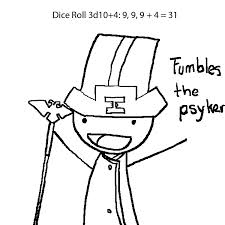
\includegraphics[width=\figwidth]{pics/9/9.png}
	\end{center}
\end{wrapfigure}
It wasn't a complete shambles, like some other exercises we'd seen, but the arbite team didn't want to be there and the psyker's aura made us all pissy. 
Little fuckups kept happening, there were some injuries, and whenever the Interrogator joined in his team would win. 


Mostly everyone blamed the training lasguns, they were utter shit and jammed on every other shot. 
There was also the fact that none of us could really get serious in a fight like this, we wanted to fight dirty and use explosives and the arbites didn't want to fight at all. 
Nothing was going right.

We all just moped around and got more and more frustrated until Sarge snapped at the psyker, who'd failed to hit anyone all day, and told him to "Do something useful damnit". 
A minute later a small localized ship-quake shook the bay and knocked crates onto both Tink and one of the Arbites. 
Then for an encore the psyker manifested a layer of ice in the floor, which he then slipped on, causing him to fly face first into the wall and knock himself out cold.

The Interrogator called a halt there and suggested that we not try this again. 
He then wandered off to see if anything was happening down on level six while we dug Tink and the Arbite out and Doc checked the psyker for a cracked skull.

Perhaps unfairly, the pysker got most of the blame for that shit-show and from then on we called him Fumbles. 
This did not seem to make him any more depressed than usual.

\begin{wrapfigure}{O}{\figwidth}
	\begin{center}
		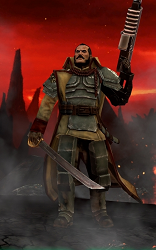
\includegraphics[width=\figwidth]{pics/9/10.png}
	\end{center}
\end{wrapfigure}
We didn't spend much time hanging around in orbit once we reached the planet. 
A shuttle brought us down to a very fancy lounge where we were greeted by the similarly posh Inquisitor who had requested our team's assistance, we'd worked with the man before and knew him by the moniker Rupert. 
Before his promotion he'd commanded two of our missions which, despite being relatively successful, had both ended with him losing an arm to what might be called excessive enthusiasm. 
We were happy to see him, between his political connections, combat prowess, and jovial demeanor he was the best direct superior we'd been given. 
Hard to understand though, he usually needed his supernaturally competent batman Alfred to act as translator and general nursemaid.

To our complete lack of surprise our new Interrogator hit it off wonderfully with the Inquisitor, both Bane and the Rupert spent the evening drinking and telling tales of ridiculous heroism. 
While they swapped stories Alfred quietly led the more serious members of our team off for a real briefing which Tink, due to his poor understanding of the standard Imperial Guard protocol of Not It, was also forced to attend; 
the rest of us joined our Interrogator for an enjoyable evening of good stories and better brandy. 


Of course before we could really get started the techie came back and dragged the rest of us into the briefing, and not because he wanted us to suffer with him or needed help taking notes and tracking our squad's responsibilities. 
As we made our way to the briefing Tink quietly asked the rest of us if Alfred had a history of cruel practical jokes and if, just hypothetically, Oak would accept 'We're Not Suicidal Idiots' as a reason for abandoning a mission.

\begin{wrapfigure}{O}{\figwidth}
	\begin{center}
		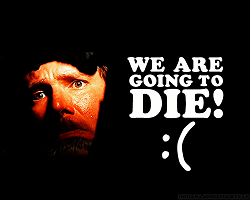
\includegraphics[width=\figwidth]{pics/9/11.png}
	\end{center}
\end{wrapfigure}
None of us had really gotten into the whole mission planning thing with the rest of the team, we figured they'd tell us anything we really needed to know when the time came. 
Doc and Sarge had taken a few peeks at the reports the adepts were putting together, but most of the info we had was from the original mission brief. 
We knew that we were fighting the Orks for this planet for some unspecified reason, we knew that things weren't going well, and we knew that something about the amount of soldiers deserting here had drawn the Inquisition's attention. 
What hadn't known was that the Rupert was the fourth Inquisitor sent here to sort things out and that two of Oak's Interrogator teams had died here as well.

Just to reiterate, this mission had already killed DOZENS of experienced inquisitorial agents and THREE full blown Inquisitors. 
One dead Inquisitor might have been understandable, but three was just ludicrous; 
the second two, at least, must have known that someone was gunning for them and they'd still been wasted without anything to show for it. 
Three of the nastiest buggers this side of Terra had come here, with their entire retinues and all their Inquisitorial authority, and died horribly; 
now it was our turn.

Of course we found it odd that the Rupert, who had all the self preservation instinct of a lemming, was still alive. 
Alfred explained that he had personally foiled over a dozen assassination attempts and that anything overt was being blocked by the Inquisitor's numerous political connections with the local brass. 
There were three regiments camped around the mansion and a pair of frigates were undergoing 'repairs' in synchronous orbit directly overhead. 
Apparently the other Inquisitors had either operated discretely and died discretely, or had demanded protection and been surprised by how quickly unpopularity can get you killed in a warzone.

Sometimes it pays to be every senior officer's cousin, schoolmate, comrade, or drinking buddy.

\begin{wrapfigure}{O}{\figwidth}
	\begin{center}
		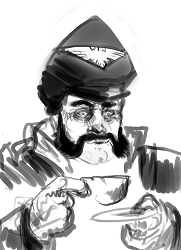
\includegraphics[width=\figwidth]{pics/9/12.png}
	\end{center}
\end{wrapfigure}
While this was all quite interesting, especially Alfred's descriptions of the messy ways the other teams had died, we were all left with a big question: 
Why the hell were we here? 
If the Rupert had managed to survive and make progress where all the other Inquisitors had died, what did he need our team for? 
None of us were happy with the batman's answer.

The Inquisitor had decided that the local guard command structure was so incredibly corrupt that he just had to sort it out personally. 
This meant that he wouldn't be able to devote his full attention to investigating the desertions, so he needed some trusty subordinates to do it for him. 
Specifically he wanted "old-sweats with conkers for dodgy business and plenty of vim, some stalwart lads who can keep mum and don't get the collywobbles when the fur flies", which apparently meant us and whatever Interrogator and teammates Oak decided to send along. 
How anyone could apply the phase "keep mum" to our Interrogator, "stalwart" to Nubby or Twitch, or "vim" to our incredibly drab teammates was a mystery, but there we were.

So while the Rupert did whatever the hell he was going to do about the corruption in the brass, we were going to be sent out to do a job that had already killed several far more competent teams. 
As Alfred outlined the largest morale and desertion problem any of us had heard of, we listened to the sound of the socialite Interrogator and the old warhorse drinking and swapping tall tales in the next room and pondered our chances of survival. 
None of us were very optimistic.

\begin{wrapfigure}{O}{\figwidth}
	\begin{center}
		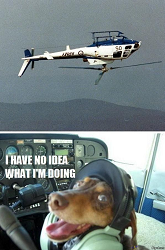
\includegraphics[width=\figwidth]{pics/9/13.png}
	\end{center}
\end{wrapfigure}
The Rupert provided rooms for our team in the mansion he'd commandeered, but we didn't get much time to enjoy them. 
Under any of our previous interrogators there would have been some intel gathering and basic plan forming, which is to say someone else would do that while we kept our heads down, but Bane didn't seem keen on sitting around. 
He burst into our rooms, wearing his damned bathrobe and neatly avoiding all of Twitch's traps, at an ungodly hour and told us to gear up for a trip to the battlefield. 
Sarge tried to ask the Interrogator just what the hell we'd be doing up at front, but the man just vaguely said that everything would work out, then wandered off before any of us could navigate the minefield in front of the door.

Less than an hour later we were all sitting in a flier, watching Tink as he frantically went through the manual and poked at the controls. 
The Interrogator sat in his seat and cheerfully deflected or ignored the frantic questions from the rest of the team about where we were going and why we were going there. 
For our part, we'd accepted that he wasn't going to tell us anything and just grabbed our usual kits and strapped in for the ride, except for Twitch, he had what might be called his 'Ork Loadout' on. 
None one sat near him and the two seats he'd piled with explosives and weapons.

After a few minutes the was a shout of success from the cockpit and the flier's engines began to warm up. 
A second later there was another shout, from the co-pilot Alfred had found for us, followed by a loud crackling sound as the nose gun went off and burned a neat hole in the side of the mansion. 
There was a short, mostly whispered argument between the two pilots and Tink came out from the cockpit, got our destination coordinates from the laughing Interrogator, then settled into the co-pilot's former seat.

\begin{wrapfigure}{O}{\figwidth}
	\begin{center}
		
\includegraphics[width=\figwidth]{pics/9/14.png}
	\end{center}
\end{wrapfigure}
As we flew Tink passed Sarge a datalsate with a tac-map of our destination, we were headed to spot supposedly just a few klicks behind our lines near one of the larger ongoing battles. 
Supposedly was the key word, Alfred or one the Rupert's adepts had shaded the whole area in and labeled it "lines partially collapsed, incredibly porous, possible desertion hotspot, expect enemy patrols and only enter in force". 


Struggling to keep the incredulity out of his voice, Sarge asked Bane why we were heading into a contested zone with only eleven men and what he hoped to accomplish. 
The Interrogator ignored the first question and told Sarge that we were going to find some deserters and, he snickered to himself here, interrogate them. 
Everyone just sort of sat there and stared at him.

The only reason Sarge didn't both start bawling him out for the sheer stupidity of this idea was that the Arbite and the two Adepts beat him to it. 
There was a long and very polite argument about how tactically sound an expedition into contested territory for no reason other than the capture of a few deserters was, especially considering that the local commissariat had put together several penal legions of them already. 
Unfortunately all the arguments and criticism just ran off the Interrogator like water, he sat there and repeatedly assured everyone that we could handle any problems and that whatever random schmuck we found would have all the information we'd need.

Sarge abandoned the discussion to go plan the landing with Tink while Doc and Nubby started pulling some extra munitions out of Twitch's piles. 
At the back of the ship the psyker morosely told everyone that he'd foreseen our horrible deaths, Twitch proceed to get into an argument with him about whether we'd all die to deserters, Orks, or Orks disguised as deserters.

\begin{wrapfigure}{O}{\figwidth}
	\begin{center}
		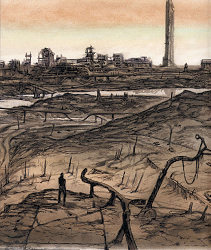
\includegraphics[width=\figwidth]{pics/9/15.png}
	\end{center}
\end{wrapfigure}
So no shit there we were heading into a combat zone, with no support, to find a bunch of heavily armed former-guardsmen then ask them why they were deserting and where they were heading. 
It really says something that it was only the third worst plan we'd been part of.

The flight got a lot more interesting as we neared the front, the ground-war on this planet was one of the bigger ones we'd seen. 
The sheer number of troops we could see below us was staggering, you could actually identify hotzones from the glow of mass lasgun fire. 
We all clustered around the windows, but after a few minutes it stopped being amazing and was just depressing. 
A near endless tide of guardsmen was marching into the fight, supported by millions of tanks and fliers, and all it was achieving was a stalemate. 
It was easy to see why desertion was a problem, the fight was bloody pointless and it was obvious that most of the soldiers sent to that front weren't going to be coming back.

The spot where we landed wasn't an active battle, it was a fairly wide valley that used to hold a fair sized town or something. 
It had been turned into a charred wasteland by artillery, the only movement we could see were soldiers standing watch up on the edges and the flash of artillery in the distance. 
It looked like the barrage was coming down right where the line was supposed to be, none of us speculated on whether they'd been allowed to pull back before the suppressive barrage was started.

Tink set us down in a dell a klick or two outside the town, or rather the loaner pilot set us down while Tink carefully watched what buttons he pressed. 
The Interrogator cheerfully reminded us that, officially, everyone left here was a deserter, so all we had to was find someone ask them some questions, then head back to base for dinner and drinks. 
We shared a pained look with the other half of the team as he bounded out the rear hatch, then followed him into the no-man's land.

\begin{wrapfigure}{O}{\figwidth}
	\begin{center}
		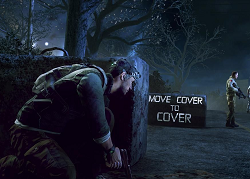
\includegraphics[width=\figwidth]{pics/9/16.png}
	\end{center}
\end{wrapfigure}
It goes without saying that the wasteland wasn't a happy place. 
None of us wanted to be there; 
even without the presence of desperate deserters or Ork scouts, anywhere that's had that many shells dropped on it is amazingly unsafe to wander around. 
Tink tried to convince Sarge that, despite the complaints from the copilot, it was his duty to stay in the flier. 
He might have pulled it off if both Nubby and Twitch hadn't joined in when they saw Sarge was actually considering it. 


As the Interrogator led us in the general direction of town in the center of the valley we kept our heads down and eyes open, the Interrogator did neither. 
The man's only concession to stealth was to occasionally sprint between wrecked buildings or walls then stand up and return to walking out in the open when he got bored. 
After the second time we just barely stopped him from stepping on an unexploded shell Sarge put Twitch in charge of walking in front of him and the rest of us spread out into a scouting permitter. 
The arbite team just walked along behind the Interrogator, mimicking his moves and quietly complaining to each other about the situation. 
It was amazing that we got the edge of the town without anyone being seen or blown up.

Not long after we entered the town proper we saw signs of life, a few small buildings were still standing and campfire smoke was coming out of one of them. 
We pulled back to discuss the plan of attack with the Interrogator, but as soon as we pointed out the building he stopped listening and ran towards it while the rest of us raced to catch up. 
We got there too late to stop him and just in time to watch as he flung the door open then stood there, with his cloak billowing around him and rosette on display, and loudly asked if anyone inside was a traitorous deserter.

\begin{wrapfigure}{O}{\figwidth}
	\begin{center}
		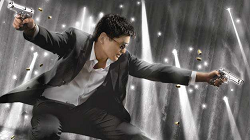
\includegraphics[width=\figwidth]{pics/9/17.png}
	\end{center}
\end{wrapfigure}
There were a few seconds of shocked silence then a rain of las-fire poured out the door, barely missing the Interrogator and clipping one of the adepts. 
Sarge and Twitch both immediately popped nades and put them through the building's windows and Nubby laid down some suppressive fire on the doorway, giving Doc the cover he needed. 
While the rest of us got the fight started and pulled the wounded adept to safety Tink stepped back, pulled down his goggles, and raised his plasma gun.

If you've never seen a plasma gun in action imagine a cross between a lasgun and a slug thrower. 
Instead of projecting a brief beam of powerful light, it gathers together an incredibly hot ball of energy then lobs it out like a stubber, but unlike a stub round that blob of plasma will burn through just about anything that gets in its way. 
Also it's bright blue, make's an incredibly ominous whine as it charges, and occasionally vents superheated gasses onto the user. 
All in all lasguns are a lot easier and safer to use, but when you want to destroy armor or punch through a wall, accept no substitutes.

Tink put several rounds through the walls on either side of the door, killing the poor bastards taking cover against them and opening firing ports for Sarge and Twitch to use. 
After that the fight was pretty one-sided, we had better positions, weapons, and training, but the real kicker was when the Interrogator came through the back door with the rest of the team. 
For all of his lack of tactical sense, the man was an impressive fighter, he swept in and wiped out the last four deserters before they managed to turn to face him, neither the arbites nor the psyker got a shot off before it was over. 
It was an impressive end to the battle, unfortunately the whole thing was spoiled a little by the wounded adept's screaming and the fact that none of us had remembered to leave someone alive for interrogation.

\begin{wrapfigure}{O}{\figwidth}
	\begin{center}
		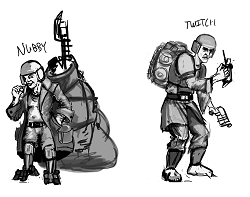
\includegraphics[width=\figwidth]{pics/9/18.png}
	\end{center}
\end{wrapfigure}
As soon as Doc was finished bandaging the adept we got away from the corpse-filled building before someone came to check out the noise. 
As we moved Bane treated everyone to a play-by-play of the fight, with sound effects, and Sarge privately decided that it would be best to keep the Interrogator away from the next group of deserters we found.

When Twitch spotted movement in another wrecked building we pulled together and formed a fairly simple plan. 
Doc, who was sticking with the wounded adept anyway, was put in charge of keeping the rest of the team out of our way. 
He led them in the opposite direction from the deserters to investigate some random pile debris, which might be hiding a secret deserter hideout or something, while the rest of us just casually walked away. 
After a little scouting and some discussion we decided that it'd probably be easier for us to pretend to be fellow deserters and ask for info than try and capture one of them.

That is to say, it was easier for Twitch and Nubby to pretend to be fellow deserters, Sarge and Tink decided to stay back and watch. 
Tink's plasma gun and other toys made him stand out a little too much for comfort and Sarge practically had SENIOR NCO tattooed on his forehead, neither of them was likely to find friends inside, but Twitch and Nubby were practically poster children for desertion. 
If a director was putting together one of those commissariat films on the evils of cowardice and asked for an obvious cretin as well as someone who'd clearly snapped a long time ago, he'd have sent both troopers back for looking too stereotypical. 
They didn't have any trouble at all walking into the camp.

\begin{wrapfigure}{O}{\figwidth}
	\begin{center}
		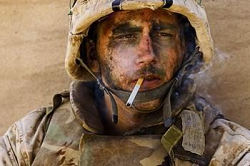
\includegraphics[width=\figwidth]{pics/9/19.png}
	\end{center}
\end{wrapfigure}
Within a minute of entering Nubby was trading lho sticks for rumors and had Twitch started collecting info on local Ork patrols. 
Of course these guys didn't know anything really useful to us, why would they? 
They were just a bunch of poor suckers who'd gotten screwed over just about everyone on either side of the war; 
none of them had any secret nefarious plan, they just didn't want to die. 


Mostly they just told us that the troopers above the valley were shooting anyone who tried to leave, which was pretty much what we expected from the commissariat, they did have one piece of interesting info though. 
One of them said that some former officer was pulling deserters together for a push out of the valley, they didn't want any part of it but we were free to try if we had a deathwish. 
Unfortunately, before Nubby could get directions from them the screaming started.

It came from the area where Doc was distracting the Interrogator and sounded awful warpy, the second it faded it was replaced with the sound of gunfire. 
The deserters all immediately ran for it and we decided to pull back to help instead of trying to stick with them. 
We commed Doc as we ran in an attempt to figure out what the hell was going on, but the medic wasn't making much sense, all we were able to establish was that someone was an idiot and Orks were involved. 


When we finally made visual contact with the team they were holed up in some rubble and exchanging fire with a bunch of deserters in another pile. 
The four of us started to flank around, but before we got halfway we were interrupted by a loud "WAAAGH" and the arrival of a squad of greenskins on the opposite side of the fight.

\begin{wrapfigure}{O}{\figwidth}
	\begin{center}
		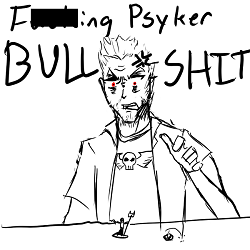
\includegraphics[width=\figwidth]{pics/9/20.png}
	\end{center}
\end{wrapfigure}
It's time like this that knowing your enemy and having a decent comms network can really pay off. 
We all grabbed cover and Sarge barked a ceasefire order to the rest of the team which, to our complete lack of surprise, was obeyed by everyone but Bane. 
Luckily a piece of debris blocked the greenskins' view of the Interrogator, which meant that the deserters were the only visible enemies. 
Following their usual insane logic the Orks all charged the hostile pile of rubble, completely ignoring us as we got into position to take out the winner. 
The fight ended without any other incidents, but once again none of the deserters survived.

While Sarge reported the small amount of information Nubby and Twitch attained, Doc filled us in on what happened. 
As he worked to patch up the second adept, the medic explained that the ruined building he'd picked for a distraction had just happened to contain another group of deserters. 
They'd been talking about something and the Interrogator wanted to listen in, so he'd led the whole team closer. 
Right as they'd got close SOMEONE, Doc threw a wad of bloody bandage at Fumbles here, decided to try listening to the deserters' thoughts instead of their voices and screwed the pooch. 
Hence the warpy scream, Doc's near deafness when we commed, and the ensuing fight. 
He said it was sheer bloody luck that Interrogator managed to dodge all the fire and hadn't wound up like Adept, furthermore it was practically a miracle that only one group of Orks had followed the noise.

All in all Doc was not a very happy trooper, despite getting a great chance to prove his medical ability, and said we'd gotten off incredibly light so far. 
He was of the opinion that it was time to cut our losses and the two bleeding Adepts seemed to agree, or at least they moaned in a sort of agreeable way.

\begin{wrapfigure}{O}{\figwidth}
	\begin{center}
		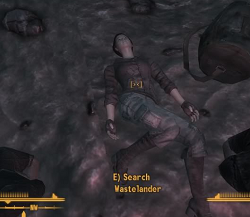
\includegraphics[width=\figwidth]{pics/9/21.png}
	\end{center}
\end{wrapfigure}
Sarge had a very weird discussion with the interrogator while Doc complained to the rest of us. 
He didn't seem to mind that we'd gone off to do our own investigation and seemed inordinately happy with the scrap of info about someone organizing the local deserters. 
When Sarge and the arbites pointed out that none of us had the slightest idea where in the large, ruined, ork-filled valley this was happening, the man only laughed and assured them that the deserters we'd just fought had probably known where it was. 
Sarge adopted the very patient voice you use when talking to slow children or armed madmen and explained that those deserters were very dead now, it was unlikely they'd be giving us directions. 
Five minutes later Sarge and Nubby were digging through the corpses looking for any "secret notes" or "maps to the hideout". 
Ten minutes later he was swearing sulphurously as he delivered the map to Bane.

Unbelievably it really was a map to where the deserters were mustering, with detailed directions and everything. 
We didn't even need to have the Adepts translate the version of gothic it was written in, the Interrogator just happened to have studied it back in the schola. 
None of us were very happy about this turn of events, for one thing it meant we weren't going to be leaving the valley yet, and for another it was complete and utter bullshit. 
Sure, occasionally you find some random thing that just happens to be exactly what you need, but it's pure luck, you don't get to depend on it happening as part of your plan. 
It was unfair that the universe was playing along with him and when it finally stopped it was probably going to get us killed along with him.

\begin{wrapfigure}{O}{\figwidth}
	\begin{center}
		
\includegraphics[width=\figwidth]{pics/9/22.png}
	\end{center}
\end{wrapfigure}
There was a lot of grumbling as we followed the map deeper into the town. 
The entire group's mood, except the Interrogator's, entered a sort of downward spiral starting at anger and transitioning through disgust to a sort of weary depression. 
While Sarge had a lot of unkind things to say about the Interrogator and most of us engaged in a sort of round-robin bitchfest with the arbites, Doc and his patients were the worst. 
He continuously whined about having to care for the two adepts who, in turn, complained about having bleeding holes in their bodies. 
We probably would have all killed ourselves before we got to the enemy if it weren't for Twitch and Tink.

Twitch, bless his paranoid little heart, accused one of the arbites of stealing his happiness and draining his very soul away. 
Tink grabbed that chain of logic and ran with it, a few minutes later we were all feeling better as Fumbles stayed a minimum of twenty meters behind everyone else. 
It was decided by fair and democratic vote that the two arbites would take turns keeping him company until Doc could get his hands on some anti-depressants for the creepy little bugger. 


The Interrogator ignored this whole charade, he was too busy walking in plain sight with the map help out in front of him. 
We figured that best case scenario his luck would hold and he'd lead us to the deserters without incident, worst case he'd get killed by a dud shell or a bunch of Orks. 
It was a win-win situation and Nubby even started taking bets on the outcome, at least until Sarge got annoyed and threatened to put him on Fumbles duty.

Unfortunately it turned out that we'd been far too optimistic.

\begin{wrapfigure}{O}{\figwidth}
	\begin{center}
		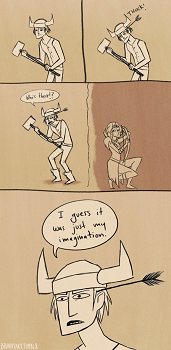
\includegraphics[width=\figwidth]{pics/9/23.png}
	\end{center}
\end{wrapfigure}
Doc was the one who first recognized the landmarks from the map, but it was Twitch who spotted the stubber nest. 
By the time we saw it the Interrogator was already half way across the killzone. 
The entire team piled up at the edge and watched as Bane walked up to a wrecked lamp-post then paused to check his map. 
Sarge frantically flipped his com to the Interrogator's channel and told him to freeze, instead he turned to face us and loudly asked why everyone had stopped. 
Everyone held their breath and waited for the stubber to open up on him.

Eventually we ran out of breath. 
Somehow the two deserters in the nest completely failed to notice that a man, in a flapping cloak that screamed "Inquisition" no less, was standing behind a post half as wide as him and talking on his combead. 
In a choked voice Sarge explained the situation, prompting Bane to lean out and stare at the nest for a few seconds then start talking in a loud stage whisper. 
This was more than we could handle, Sarge peeked around the corner and verified that the hostiles looked like real soldiers and neither one was blindfolded, then jerked back as the stubber swung to bear on him. 
We all heard one of the deserters tell the other that he might have seen something.

Sarge, Doc, and the Arbites started to argue over their coms with the Interrogator, who was whispering so loudly that we could all hear him from across the street, while the rest of us got into a fairly heated discussion about just what the hell was going on here. 
Tink was of the opinion that something warpy was happening, though Fumbles denied this and claimed that everything was normal. 
This prompted Nubby to start blaming the depressed psyker for "screwin wit da laws of fisiks", while Twitch, of course, blamed everything on the Orks. 
The argument came to a crashing halt when Tink's voice rose almost to same level as the Interrogator's and the stubber opened up on our cover.

\begin{wrapfigure}{O}{\figwidth}
	\begin{center}
		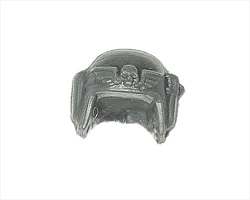
\includegraphics[width=\figwidth]{pics/9/24.png}
	\end{center}
\end{wrapfigure}
It wasn't a long or well aimed burst, just a spray across our general area. 
In our professional opinions these guys were obviously more interested in convincing us to leave than actually scoring a kill, but a freak ricochet managed to nail one adepts in the leg. 
While Doc opened his medkit for the third time that day and Nubby yelled abuse at the two deserters, Twitch directed our attention to Bane. 
He was briskly walking into the alley the nest was guarding while the enemy was distracted. 


We figured he was going to take out the stubber nest so we could follow him in, instead he commed us all. 
In a voice that just oozed smugness he ordered us to meet him in the main courtyard, then said he was "going dark" and turned off his combead. 
Hopefully he heard what Tink yelled at him, the deserters certainly did, a second ricochet lodged itself squarely in Twitch's helmet.

Everyone except Sarge and the Arbites was in favor of ditching the Interrogator and heading back to the flier, unfortunately orders were orders and we had a job to do. 
After all of us calmed down we pulled back to a more secure wrecked building and got a plan together. 
Shooting our way in was out of the question so we needed a way to sneak in, the problem was that none of us were very sneaky and only half of us stood a chance of impersonating deserters. 
We didn't have spare uniforms for the arbites and neither adepts was up for anything strenuous; 
Fumbles volunteered to make us all invisible, but Doc immediately vetoed that idea and sent back to his corner on the far side of the building. 
In the end we decided just to leave them all together to act as a secure base while we went in ourselves.

Tink's toys and plasma weapon were crammed into a rucksack, Doc was pushed into a puddle of mud, and Sarge hoped really hard that no one on perimeter duty had a grudge against NCOs. 
Nubby and Twitch in the lead, we went to back-up the idiot.

\begin{wrapfigure}{O}{\figwidth}
	\begin{center}
		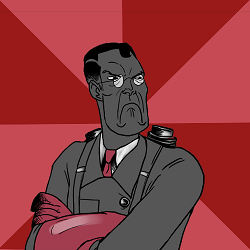
\includegraphics[width=\figwidth]{pics/9/25.png}
	\end{center}
\end{wrapfigure}
We circled around to another entrance in hope of finding some less weird guards than the selectively blind ones that'd shot at us. 
The main entrance to the deserters' compound had at least two gunners covering it and a few troopers lounging around in front of it. 
A protesting Nubby was kicked out ahead of us to act as emissary and sidled up to the troopers with his hand held comically high in the air. 
None of us heard what he told the guards, but they quickly lowered their weapons and let Nubby join them at their post. 
Lho sticks were exchanged, a bottle materialized from somewhere, and after a few more minutes than were probably necessary he called us over.

Nubby made a round of introductions, starting with Sarge, who got a long appraising look from the man in change, and ending with Doc. 
When the desters saw we had a medic they perked up and started asking pointed questions about the state of his medkit, i.e. 
how many ampules of painkillers he had and how many he really needed. 
Doc shot Nubby a glare and ponied up about a third of his supply, this immediately made us several new friends and one of the troopers happily agreed to show us around. 


The tour consisted of a meandering walk through the collapsed buildings that made up the compound, and ended in an open central area populated by a few dozen deserters. 
He dumped us on an oddly cheerful man, who welcomed us to the "First Free Army" and informed us that we were extremely lucky. 
It turned out we'd arrived just in time to hear an important announcement from the general, after it was over he'd see about getting us fit in, but for now we should just listen. 


A pair of men who could've been Sarge's brothers came out of a nearby building and started barking everyone into formation. 
As we shuffled around Twitch spotted a single soldier wearing a Valhallan coat and hat, a preposterously large mustache, and a dozen things which obviously marked him as an Inquisition agent.

\begin{wrapfigure}{O}{\figwidth}
	\begin{center}
		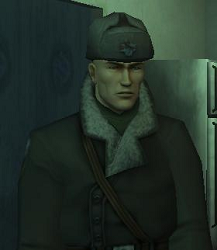
\includegraphics[width=\figwidth]{pics/9/26.png}
	\end{center}
\end{wrapfigure}
Sure the greatcoat covered most of him and the moustache looked amazing, but anyone who looked closely was going to bust him. 
He'd actually holstered his mastercrafted silenced auto-pistols outside of the coat and you could even see his rosette peaking out of the front of the coat, it was like he wasn't even trying. 


We quickly moved in around him and blocked everyone's view while Sarge did his best to fix Bane's disguise. 
Nothing could be done about the shiny carapace greaves and boots, but the autos were stashed in his pockets and replaced with a spare laspistol, the rosette was tucked inside his shirt, and we managed to shove him into parade rest before one of the sergeants came over to yell at us. 
Our squad was split up onto either side of the Interrogator and we all did our best not to draw attention. 
As the last deserters formed up, a big man wearing a general's insignia tacked onto a major's uniform came out and addressed the troops.

As moving speeches go it rated a solid seven; 
hitting several key topic like the importance of camaraderie and the mating habits of commissars, but losing a few points for talking too much about protecting civilians. 
Also for being a traitorous heap of lies designed to sap the fighting spirit of brave guardsmen and lure them into vile heresy. 
After everyone had been suitably pumped up he moved onto some real topics, like the rumors that some Rogue Traders were trading trips off planet for favours or a gig of service in their private armies. 


Apparently these rumors were not only completely true, but the General had managed to contact one of them and worked out a rendezvous, at this point he flourished a calligraphy filled note and there was a great deal of cheering. 
Furthermore, he'd made contact with a sympathetic regiment which would turn a blind eye to our escape from this hellhole, but before he'd go into details he needed to make sure no one here was a commissariat spy.

\begin{wrapfigure}{O}{\figwidth}
	\begin{center}
		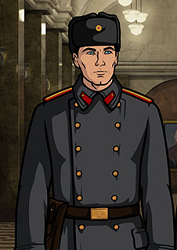
\includegraphics[width=\figwidth]{pics/9/27.png}
	\end{center}
\end{wrapfigure}
While the General explained that he'd heard reports that an unmarked flier had landed in the area and listed all the horrible things that the commissariat would do if it found us, his two henchmen started traversing the line of deserters. 
They carefully went over each man, occasionally asking them questions or inspecting their equipment. 
We all nervously checked ourselves over and eyed the Interrogator, who'd apparently gotten tired of standing straight and was now in a pose best described as 'lounging'. 
As the inspectors worked closer he took out a lho stick, jammed it under the fake moustache, and drew out his trainee rosette. 
We watched in horror as he flipped off the top and lit his lho stick with it.

Just to be clear here, the man had a LIGHTER installed in his INQUISITORIAL BADGE OF OFFICE. 
Emperor knows why he had it done or how he got someone to agree to fiddle with the thing, but he used it right there in the middle of the deserter base, then dropped it back down his coat. 
It sat there and peeked out the front like a poorly camouflaged trainee on guard duty. 
Both Doc and Sarge frantically whispered at him to put it away, but Bane just stared at them blankly and before the point got across the two henchmen reached us.

Twitch passed review without comment and they actually stepped back a bit when they reached Nubby, his unique odor could affect people like that, Tink didn't get off so easy though. 
Whether it was his bulging pack, fancier than usual armor, or near permanent expression of petulance mixed with superiority, something about him bothered the inspectors. 
One of them stepped behind the techie and flipped open his pack, exposing his stash of gadgets and the bulky plasma-gun. 
The other goon smiled a shit-eating grin and loudly asked the General what sort gear a "slimy little commissariat weasel" would carry.

\begin{wrapfigure}{O}{\figwidth}
	\begin{center}
		
\includegraphics[width=\figwidth]{pics/9/28.png}
	\end{center}
\end{wrapfigure}
Tink's panicked denials and the supporting testimony from Nubby and Twitch might have gotten him off the hook if he had kept a level head, but when they took his pack away he exploded in impotent nerd-rage. 
While he showed a lot of passion and his word choice was quite inventive, Tink was a lousy melee fighter and his pathetic attack didn't impress the henchmen. 
They quickly subdued him and he was dragged off for questioning by a pair of deserters.

While everyone watched Tink's beatdown each of us evaluated our options. 
We could all see that there wasn't any way we'd survive a straight fight in the middle of this place, our only real chance was to keep up the disguise until we could do something sneaky. 
The problem was that there didn't seem to be any way the Interrogator would pass inspection and there was no way of knowing what he'd do when they spotted him. 
If they just captured him like Tink we'd be able to try and spring them both together, but they could just immediately execute him or he might start a fight and drag us in. 
Each of us was so busy agonizing over this that we almost missed it when Bane made is move.

The Interrogator just casually walked from his position in line just past Tink, to a spot between Nubby and Twitch. 
Apparently everyone was too busy watching our mouthy techie getting the shit beat out of him to notice, when the inspection resumed both goons moved onto Sarge and Doc without blinking. 
It was really quite amazing, the man hadn't done anything sneaky, he'd just chosen the exact moment when everyone was distracted. 
We all did our best to keep the surprise off our faces as the inspection was wrapped up without further incident.

\begin{wrapfigure}{O}{\figwidth}
	\begin{center}
		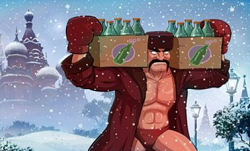
\includegraphics[width=\figwidth]{pics/9/29.png}
	\end{center}
\end{wrapfigure}
Secure in the knowledge that no spies were present, the General outlined a complex plan for escaping to the rendezvous with the trader. 
There were a lot of regiment names, passphrases, waypoints, and other stuff we really didn't care about, then the parade was over. 
As the other newbie deserters walked off to do whatever it was they did around here we quickly pulled together to hash out a rescue plan. 
Unfortunately the Interrogator didn't have any time for that, he made a beeline for where the General and his goons were talking with a few of the recruits.

Sarge and Twitch went off to rescue Tink, leaving Doc and Nubby behind in the square. 
Their job was to grab the Interrogator and convince him not to do anything suicidal until Sarge returned, in Doc's opinion this was not an ideal plan, but there hadn't been time to think of anything better. 
Both troopers hustled after the Interrogator and got there just as he reached the group of chatting deserters. 
They watched in horror as Bane, hand outstretched and fake mustache bristling, Interrogator walked right up to the General and greeted him in a horrible Valhallan accent.

What followed was string of stereotypical and cliched comments that would've mortally offended any actual Valhallan. 
Both Nubby and Doc had served with the iceworld regiments before and it was physically painful to hear the interrogator calling everyone comrade, joking about how hot the climate was, and complaining lack of alcohol in the camp. 
It was lucky that a deserter's hideout is the last place you'd find a real valhallan and incredibly lucky that no one here knew that or, apparently, had ever met one. 
The General welcomed "Ivan Ivanov" with a smile, laughed at his jokes, and promised he'd go far in the First Free Army. 


Doc and Nubby had about a second to feel relieved, then the General spotted them. 
His smile turned into a suspicious glare and he asked Doc just which regiment he was from.

\begin{wrapfigure}{O}{\figwidth}
	\begin{center}
		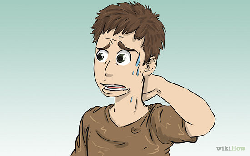
\includegraphics[width=\figwidth]{pics/9/30.png}
	\end{center}
\end{wrapfigure}
Doc was a clever boy, a good fighter, and a decent medic, but he was a terrible bullshitter. 
He froze up for a solid five seconds then started stuttering, asking if the General meant him and if he really wanted his whole life story. 
When the General didn't stop glaring the panicking medic took refuge in the truth, and started to rattle off the regimental details of the Gener 99th Medium Infantry, a regiment which had died years ago. 
Nubby tried to come to the poor boy's rescue, but the General responded in the way that most officers did when confronted with Nubby Nubbs, which is to say he ignored the little trooper in hope that he'd go away if no one gave him any attention.

Eventually the steam of babble was cut off and the General started asking some very pointed questions. 
Doc scrambled to field these, but was distracted by the Interrogator. 
Bane had wandered behind the General, and was carefully scrutinizing the note that he'd been waving around when talking about contacting a Rogue Trader. 
After giving it a good once-over, the Interrogator held up his wrist-chrono and fiddled with it until a screen and lens popped out the sides. 
A mesh of green light was projected on the note as he carefully scanned the whole thing, both sides. 
Doc could barely keep his eyes off the scene of blatant spying as he fumbled through the questions, if anyone even glanced towards the Interrogator they'd all be killed.

\begin{wrapfigure}{O}{\figwidth}
	\begin{center}
		
\includegraphics[width=\figwidth]{pics/9/31.png}
	\end{center}
\end{wrapfigure}
No one did look though, everyone was busy staring at Doc who had already sweated out half his-body mass and was going for three-quarters. 
He just barely managed to answer all the questions aimed at him without blurting out something about working for the Inquisition, but it was obviously just a matter of time before he either tripped up or fainted. 
Right as things reached their most dire the Interrogator finished, walked up to Doc, and threw an arm around his shoulders. 
In that horrible accent he chastised the General for being too suspicious of "bosom companion Comrade Doctor-Boy" then told a series of horribly cliched jokes.

Just like that everyone was all smiles again. 
The General stated that any friend of Ivan's was a friend of his then shook Doc's damp hand and went to talk to some other recruits. 
Doc practically collapsed in relief and Nubby grumpily swore at them both from the puddle he'd been shoved into by one of the goons when he wouldn't shut up. 
The three of them headed in the direction Tink had been taken and Doc pulled out his combead. 
Before he could call anyone the air was filled with Twitch's screaming and, on reflex, both soldiers hit the dirt, dragging the Interrogator down with them.

\begin{wrapfigure}{O}{\figwidth}
	\begin{center}
		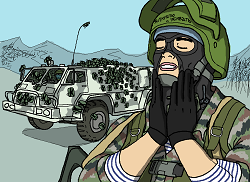
\includegraphics[width=\figwidth]{pics/9/32.png}
	\end{center}
\end{wrapfigure}
Twitch was having a pretty good time, sure he was in the middle of a hostile base inside an orc-infested battlefield, but Sarge had given him one of those good orders. 
He'd been told to "make a distraction, a big one". 
About half of his supply had been secreted around the base, no one had even commented as he'd walked around holding the explosives, and the only troopers that had seen him planting them had backed away when he asked them if they wanted to help. 
He figured it'd take just long enough for everyone to figure out the situation for them to get safely out of the base. 
With a big smile on his face, Twitch sat and waited for Sarge's signal. 


When his comm clicked the demolitions trooper took a big breath, screamed "INCOMING ARTILLERY", and hit his first detonator. 
The shout was reflex-echoed by several deserters and the entire base started shaking with well timed and placed explosions. 
A few seconds after the first barrage Sarge's voice came from his combead, instructing everyone to head for the side exit Bane had used. 
Twitch smiled and touched his dented helmet as the second barrage removed a certain stubber nest. 
It was a very good day.

\begin{wrapfigure}{O}{\figwidth}
	\begin{center}
		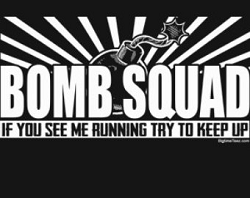
\includegraphics[width=\figwidth]{pics/9/33.png}
	\end{center}
\end{wrapfigure}
The squad came back together as they all made for the same exit. 
Tink was walking on his own, but Sarge was carrying all his gear. 
Doc slapped him with a stimm, just to be on the safe side, and eyed Sarge who was half covered in blood. 
The Interrogator asked how he'd sprung the techie and Sarge just stared back, glanced at the chain bayonet he was still holding, and gruffly said that he'd explained the Chain of Command to Tink's new friends. 
Both Nubby and the Interrogator broke into rather tactless laughter, until we all saw Twitch coming in at a dead sprint.

None of us stopped to ask why Twitch was running, it's not a question you ask demolitions experts, you just do your best to keep up with them. 
As we cleared the city a final barrage collapsed our exit, crushing a few deserters who'd been hard on Twitch's heels. 
Sarge commed the other half of the team and told them to get ready to bail, then we all just focussed on running.

We were almost to the arbites when the deserters launched their pursuit. 
A dozen ex-guardsmen took turns chasing us and taking potshots at our backs and behind them a salamander burst through a wall then turned to face us. 
The General himself was standing out of the top hatch and blasting at us with a pintle-bolter while yelling at his troops to run faster.

We got a few shots off as they closed and the Arbites laid down some decent covering fire, but keeping to cover was slowing us down and the salamander steadily gained on us. 
Both the mines Twitch dropped behind us were easily dodged by the salamander's driver and as we reached the arbites it became apparent that we'd have to at least disable the vehicle if we wanted to escape on foot.

\begin{wrapfigure}{O}{\figwidth}
	\begin{center}
		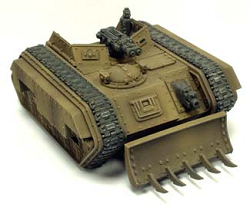
\includegraphics[width=\figwidth]{pics/9/34.png}
	\end{center}
\end{wrapfigure}
We got into cover as the enemy closed and tried to pick off some of the deserters. 
We didn't have much luck since most of them were smart enough to use their own cover, but Bane managed to nail three of them with his autopistols, the man was an amazing shot if nothing else. 
No one managed to hit the General and as the salamander got closer we all scrambled for heavier cover and got ready to surround the vehicle.

If we'd had more time or space one of Twitch's mines would've been perfect, but the overcharged plasma bust Tink put into the vehicle's side armor was a close second. 
He managed to get the engine on his first shot completely immobilizing it and making it much easier for us to snipe at its firing ports. 
The General saw the situation was desperate and started to wildly swing his bolter around, hosed fire at us while we all tried to land a shot on him. 


Doc and Sarge both missed their shots and the rest of the squad stayed in cover instead of taking the chance. 
The Interrogator and one of the Arbites didn't bother with cover, preferring to nimbly dodge through the bolter rounds and get shot in the face respectively. 
Behind the salamander Fumbles peeked out of a doorway and raised his hands towards the General, we all ducked down and prayed. 
There was a titanic BANG and the world went white for a few seconds, only Sarge saw as the Interrogator leapt up onto the Salamander, put a gun against the stunned man's head, and mutter a pithy one liner before blowing it off.

\begin{wrapfigure}{O}{\figwidth}
	\begin{center}
		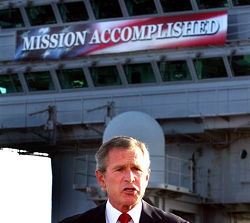
\includegraphics[width=\figwidth]{pics/9/35.png}
	\end{center}
\end{wrapfigure}
Once everyone could see again we finished off the last deserters in the salamander without incident, unless you call Tink overheating his plasma gun and dropping it on his foot an incident. 
The important thing is that no-one else died and the other deserters legged it after salamander was dealt with. 


The end count was two dead (one of the adepts died while we were away), two wounded, and one very unconscious psyker. 
The Interrogator said we weren't allowed to just leave him, so Sarge carried him while the arbite carried the adept. 
The two dead were given a proper military cremation courtesy of Tink's plasma gun, which he managed to overheat and drop on his foot a second time during the quick service.

That done with we all headed back for the flier, which the copilot confirmed was still completely secure. 
As we walked the Interrogator congratulated everyone on killing a dangerous rebel and helping him secure a piece of critical information. 
He happily told everyone how the information we'd found identified both treacherous Rogue Traders and traitors within the local guard command, it was sure to be a key part of our investigation. 
While it really was a good haul, especially for how stupid the whole mission concept had been, most of us just ignored him and Tink actively glared at him while muttering about how unfair the universe was.

When we got back to the flier and anger towards the Interrogator was redirected towards the copilot, who had failed to mention the two other fliers or the woman holding a gun to his head.

\begin{wrapfigure}{O}{\figwidth}
	\begin{center}
		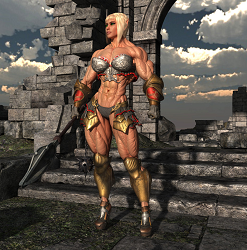
\includegraphics[width=\figwidth]{pics/9/36.png}
	\end{center}
\end{wrapfigure}
Since none of them shot at us, we decided the situation was some sort of political and deferred to the Interrogator. 
Bane ignored the men stepping out of the other fliers, knocked on the woman's door, and actually held up a hand to help her down when she opened it. 
To our amazement she actually took it and laughed a little as she stepped down, all two plus meters of her.

To put it simply the woman was huge, in several ways, and while she might have been beautiful we were all too focused on the fact that she was bigger than Sarge and had more scars than all of us put together. 
She was carrying an astartes sized bolter, had an eyepatch shaped like a heart, and was wearing what had to be a custom made set of carapace armor. 
The interrogator was a head shorter than her and had the sort of grin you see on professional mountaineers or big-game hunters.

None of us could hear what the two said to each other, though it was apparent that our boy was doing well. 
We heard a few laughs that sounded like a leman russ gunning its engine and if any of us had put our hand where he did we'd have lost them and the arm too. 
After a while Bane called us over, introduced the woman as Ivana Krushyu, and told us that she represented a very influential man who wanted to meet us. 
We all got in the flier, Tink didn't argue when Ivana took his seat in the cockpit, and headed off to meet the man who was very politely taking us prisoner.

\begin{wrapfigure}{O}{\figwidth}
	\begin{center}
		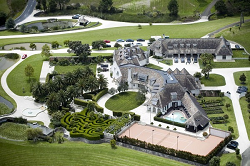
\includegraphics[width=\figwidth]{pics/9/37.png}
	\end{center}
\end{wrapfigure}
Since none of us had anything better to do we all followed Fumbles' example and took a nap during the flight. 
This meant it was a bit of a shock when we woke up in some villa with a few dozen guns in our faces. 
We were relieved of our weapons by some of the hardbitten men around us, who might as well have been wearing shirts that said "Deserter Mercenaries", and this time Tink kept his mouth shut when his plasma gun was taken away.

Fumbles was still out of it, so Sarge carried him as we were herded to rather nice waiting room. 
Ivana and the Interrogator ditched us there, presumably to talk to the boss without us guardsman dirtying the place up. 
They took half the guards with them and this evened the odds to the point where some of us started to get ideas.

The men who'd disarmed us hadn't been nearly thorough enough. 
Doc only had his medkit and Tink had nothing, but Sarge still had his boot-knife, Nubby had a stubgun, and Twitch had his backup-backup grenades as well as laspistol. 
Even if the rest of the team and the copilot had nothing we had enough firepower to take the guards and after that we'd have their shiny combat shotties. 
On top of that we could see the flier sitting on its pad just a short sprint away, there was a real chance that we could escape and even ditch the Interrogator in the bargain. 
It was very tempting, but none of us wanted to leap into action and risk getting killed yet. 
Except for Twitch no one was absolutely sure that these guys were planning to kill us, after all they could have just done that back in the valley.

Then we overheard one of the guards asking another if the boss was planning to kill us personally like the other Inquisition goons.

\begin{wrapfigure}{O}{\figwidth}
	\begin{center}
		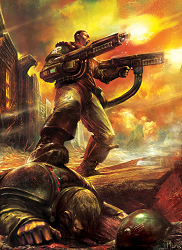
\includegraphics[width=\figwidth]{pics/9/38.png}
	\end{center}
\end{wrapfigure}
Doc acted as the distraction, he spilled half of his medkit and a few of the less scrupulous guards noticed several ampules of very expensive drugs rolling past their feet. 
During the brief scramble Sarge buried his knife in one guard's throat, Nubby plugged another in the gut, and Twitch scored a headshot, leaving just four guards. 
It was strategy, not luck, that all the guards were closer to the arbite and adept than the rest of us and while neither had a weapon they were both able to tie up a guard and melee for a second. 
Unfortunately that left two guards free. 


The first shot barely missed Doc as he scrambled for cover and the second caught the arbite in the side where it was mostly stopped by his armor. 
Those two shots were all they got, because Tink grabbed one of the falling shotguns before it hit the floor and everyone else was already switching targets. 
Within seconds all the guards were dead in exchange for a single nasty wound on the arbite and a broken arm on the adept. 
It was a good trade all in all, but we could hear reinforcements coming.

Twitch's two nades kept the incoming guards back while grabbed our shotguns and made an exit. 
There hadn't been any guards near the flier when the fight started, which mean that the copilot was free to sprint to it while the rest of us followed more slowly. 
The first hostiles came in from the wrong side and got fried by a quick burst from the flier's nose gun, but the second set came from behind it and engaged us in a running firefight. 


There was no cover to speak of on the path to the flier, it was going to be a bloodbath unless we were exceedingly lucky. 
Just this once we were.

\begin{wrapfigure}{O}{\figwidth}
	\begin{center}
		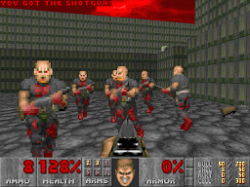
\includegraphics[width=\figwidth]{pics/9/39.png}
	\end{center}
\end{wrapfigure}
None of us had paid much thought to Fumbles. 
We certainly didn't want to carry an unconscious body with us as we ran, so we had left him to the arbite and adept to worry about. 
He was awake now though, and for the first time since we met him he didn't fuck up. 
The psyker waved his hands and one of the incoming guards turned around then hosed his squadmates with point blank, automatic shotgun fire. 
It was pretty gruesome.

Some of the guards got shots off at us before they died, taking a chunk out of both Nubby and Sarge, but not doing any serious damage. 
The same couldn't be said for the fire that came in from our pursuers though, their first volley blew the adept to pieces and forced us all to duck and return fire instead of continuing our sprint. 
The going got much slower after that, becoming a fighting retreat instead of an all out run, we were still making progress though and could hear the flier's engines spinning up. 


Unfortunately we weren't the only ones who noticed the flier getting ready. 
When we were about fifteen meters from it, a rocket lanced out of the entrance. 
We watched in horror as the rocket went right through the windshield, then the copilot, and went off in a fireball that killed our only real chance of escape.

\begin{wrapfigure}{O}{\figwidth}
	\begin{center}
		
\includegraphics[width=\figwidth]{pics/9/40.png}
	\end{center}
\end{wrapfigure}
That was pretty crushing to tell the truth, but we decided to fight on anyway. 
What else was there to do? 
We found some decent cover around the landing pad and dug in like proper guardsmen.

Between our shotguns and another well placed body-puppet spell we killed another dozen guards and convinced the rest that we were above their pay-grade for the time being. 
There was a nice lull which Doc used to patch everyone up, without painkillers may I add, and Nubby used to scrounge ammo from some of the closer corpses. 
After that we just sat around and got ready for them to bring in the heavies and kill us.

There wasn't another attack though, instead we heard a familiar voice telling us to stand down. 
The Interrogator came out of the main entrance with Ivana at his back, holding her bolter and with a rocket launcher slung over her shoulder. 
Bane alternated between congratulating us on our bravery and yelling at us for acting without orders, then segued into a lecture on how everything was being worked out and we all might come out of this alive if we put down our weapons and acted intelligently. 


The vote was four to two in favor of just shooting him until Sarge put his foot down and told us to surrender.

\begin{wrapfigure}{O}{\figwidth}
	\begin{center}
		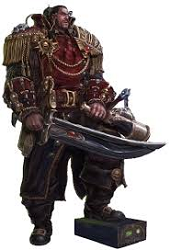
\includegraphics[width=\figwidth]{pics/9/41.png}
	\end{center}
\end{wrapfigure}
The time the weapon search was very thorough and an untouchable was brought up and handcuffed to Fumbles. 
Once we were all subdued a man in a ridiculously gaudy overcoat came out to gloat at us a little. 
Well really it wasn't just gloating, there was a fair bit of praise mixed in. 
He seemed genuinely impressed with the mess we made and went so far as to offer us jobs in his personal guard. 


This was actually a pretty attractive offer, especially after the Arbite claimed he'd rather die than betray his duty, then did. 
There's a moral in there somewhere about pointless bravado.

The Trader put his bolt pistol back in its holster then ordered his men to take us away to think things over. 
As we were bundled off Tink and Doc noticed that, for once, the Interrogator wasn't talking or flirting. 
Instead he looked rather ill and actually stumbled over his own feet and fell when the trader slapped him on the back. 
Doc put it down to having one of his teammates executed in front of him, but Tink formed a suspicion which he shared with Twitch during the walk to the cells.

We were all, except for Fumbles, given one cell to share. 
It was really quite nice of them not to split us up and the cel wouldn't have been too bad if it had more than two bunks. 
As it was we made ourselves as comfortable as possible and mulled over the situation. 
That is to say, Sarge and Doc mulled over the situation, Nubby just went to sleep while Twitch and Tink excitedly whispered about something.

\begin{wrapfigure}{O}{\figwidth}
	\begin{center}
		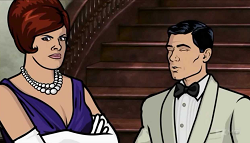
\includegraphics[width=\figwidth]{pics/9/42.png}
	\end{center}
\end{wrapfigure}
After a few hours Bane showed up with Ivana at his side. 
The valkyrie wasn't in her armour this time, instead she was in a dress that reminded Sarge of the storage tarps you put over tanks. 
It was hard not to notice the way she kept looking at the Interrogator, who had his arm wrapped around her waist.

For his part Bane was obviously drunk. 
This never seemed to impede him much, instead it just make him annoying happy. 
He cheerfully informed us that the Trader had agreed just to imprison us here for a few months while he finished his business on the world, after that we'd be free to go about our business. 
Furthermore Bane promised to come visit us regularly and maybe get us a bigger cell after a few days. 
Our massed glares just sort of bounced off his drunken cheerfulness.

His message delivered, Bane bade us good night and, as a sort of afterthought, handed us the amasec bottle he'd been carrying. 
Ivana chimed in at this point and told that this was an incredibly generous offer that was only being given to us thanks to our handsome and charming boss. 
This triggered a round of flirting that was outright sickening. 
Equal parts cheesy and repulsive, it just kept going and going while we looked on in disgust. 
He just spouted line after horrible line, which she ate up then returned with overtones of horrible crushing. 
Honestly we weren't sure who was worse, they both were acting brain-damaged and the horror show only ended when Doc and Twitch started gagging.

Bane shot us a glare for interrupting and led his lady away, as he left Tink ran to the edge of the cells and watched carefully. 
The techie started cackling with glee when he spotted the Interrogator stagger for a few steps after passing one of the other cells. 
Tink's fascination with our drunken Interrogator was only the second most interesting thing in the cell though, as Nubby grabbed the bottle of amasec its label slid off. 


There was writing on the inside.

\begin{wrapfigure}{O}{\figwidth}
	\begin{center}
		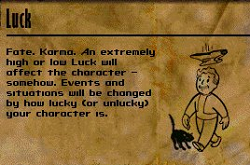
\includegraphics[width=\figwidth]{pics/9/43.png}
	\end{center}
\end{wrapfigure}
The note explained that Bane had "seduced a high level subordinate to our cause" who had confirmed the presence of high ranking traitors in the Imperial Guard. 
Furthermore the traitors would be arriving tomorrow and we'd be taken out for exercise as they arrived. 
Our gear would all be provided and the guards present would be working with us. 
As long as we were ready we'd be able to take out the traitors and escape all at once.

It'd be an understatement to say we were surprised. 
Assuming it was all true the bastard had actually come through for us, the plan sounded relatively solid and if we pulled it off it'd turn a pretty abysmal failure into a major victory. 
The problem was that none of us could see how he'd done it, except for Tink that is.

Tink and Twitch's excitement boiled over when we read the note and they let us in on their secret. 
According to them our Interrogator was a powerful psyker or possibly a vampire ork. 
Of course this was rejected by Nubby on the grounds that Bane hadn't exploded, summoned any daemons, or gone some variety of crazy during the mission. 
Tink claimed that most psykers didn't do these things, but had a great deal of difficulty convincing anyone. 
Especially when Fumbles was brought up as an example.

His theory went that the Interrogator was some sort of nascet, which we took to mean sneaky, psyker who used his powers to make himself incredibly lucky. 
Furthermore, Tink claimed he did this by stealing other people's luck, which was why things kept going to shit for us, but not him. 
This was a compelling theory and was backed up nicely by the way he acted around the untouchable and how Fumbles had always screwed up so massively around him. 
At this point Twitch reiterated his theory of vampire ork as opposed to sneaky psyker, but didn't manage to convince anyone.

Before we went to sleep a plan was hatched and that night we had some very strange dreams.

\begin{wrapfigure}{O}{\figwidth}
	\begin{center}
		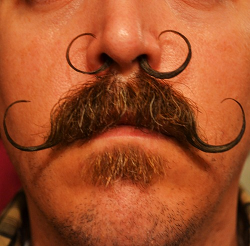
\includegraphics[width=\figwidth]{pics/9/44.png}
	\end{center}
\end{wrapfigure}
Every single one of us dreamed of a massive nose and mustache which bellowed "Alfred is this blasted thing on?" It was followed by a weary voice informing him that the 'thing' was fifth company's psyker and he didn't need to shout.

After a little more arguing the Rupert finally backed up to where we could fully see him, but he still yelled. 
We noticed that the Inquisitor had traded his dress uniform for a set of power armor and had definitely seen battle recently. 
Behind him Alfred was busily relaying orders to several subordinates we couldn't make out and there was the sound of fighting nearby. 
Sarge tentatively asked what was going on and the Rupert clapped his hands in delight.

What followed was a rather bewildering briefing on the current state of the war. 
Apparently the Rupert had claimed command as Inquisitor General and was in the process of bloodily purging anyone who argued while simultaneously fighting off a major Ork attack. 
He seemed quite happy about the whole thing, a nice change of pace he said, the only 'spot in the mustard' was that man on the top of his list, Lord General Ourumov, had 'done a runner'. 
He'd apparently left his post to visit some Rogue Trader and the strike team had missed him, by any chance did we know where he'd run off to?

Sarge was proud to report the we were inside the Trader's planetside base and were, in fact, already planning our ambush on the traitors. 
This pleased the Rupert immensely, but Sarge ran into trouble when he asked for the Trader's name or location so he could send reinforcements. 
Everyone did their best to remember and completely failed, only managing to offer some details about the landing pad area and the name of one subordinate. 
It only got worse when Nubby admitted that we were all actually prisoners, the Rupert wasn't fazed, but we could see Alfred wince in the background.

At least we were able to say that our Interrogator was not only walking around free, but actively 'suborning' the enemy.

\begin{wrapfigure}{O}{\figwidth}
	\begin{center}
		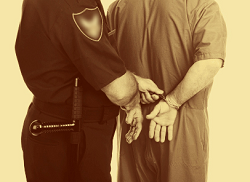
\includegraphics[width=\figwidth]{pics/9/45.png}
	\end{center}
\end{wrapfigure}
In the end the Rupert vowed to do his best to pinpoint us using this "damned warp mumbo-jumbo", then went off to see who was shooting holes in his wall with a sniper rifle. 
Leaving us in a sort of awkward collective dream which became progressively weirder until Doc managed to wake up give everyone a good kick. 
None of us were able to look at Tink without feeling uncomfortable for a while after that and we all felt sorry for Twitch. 
No one should have to spend their entire night being continuously ambushed by Kommandos, especially not ones wearing maid uniforms and sporting mechadendrites.

In the morning a shift of guards came for us and, as promised, they didn't actually lock our cuffs. 
Similarly, when we picked up Fumbles we all felt the weight of his aura as the replacement Untouchable activated a limiter. 
A whispered word from Doc stopped the psyker from starting a bloodbath the second his powers were returned and we all followed the guards through the villa. 
While Sarge quietly went over the arrangements with the guard captain and Doc brought Fumbles up to speed, the rest of us sized up the untouchable. 
We had plans for him.

Our "exercise area" was a large courtyard with a fountain at one end and a landing pad at the other. 
There were a few guards standing near doorways and some more on the roof, our escort warned us that these guards were not friendly. 
Bane and the valkyrie were waiting near the fountain, next to a row of flower boxes which poorly concealed all of our gear. 
The Interrogator was in costume again, he'd replaced his coat with one that matched the guards and gotten a hat too. 
Once again his rosette was visible just sticking out of the front of the coat, none of us commented on this.

\begin{wrapfigure}{O}{\figwidth}
	\begin{center}
		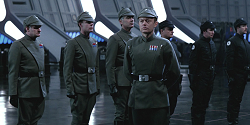
\includegraphics[width=\figwidth]{pics/9/46.png}
	\end{center}
\end{wrapfigure}
We lined up within easy grabbing range of our weapons while the Interrogator explained the final details of his brilliant plan. 
The traitors and their "foul xenos master" would be arriving shortly via shuttle and we'd be presented to them as a token of goodwill and proof of the Trader's competence. 
We'd be lined up right in front of our weapons and as they came to inspect us and gloat he and Ivana would move behind them. 
When he gave the signal we'd seize our weapons and kill their personal guards while our escort attacked the guards around us. 
After the guards were all dead we'd take the traitors prisoner, all pile into the shuttle, and escape while a distraction kept off any pursuit.

It sounded like a solid-sounding plan and except for a few additions of our own, we intended to follow it. 
The Interrogator walked over to the landing pad, a few of Ivana's guards split off to get into position, and we made what preparations we could without tipping off either set of guards. 
Before long a standard issue guard shuttle landed in the courtyard and a half dozen men in uniform got out, they were followed by a tall, thin figure in a cloak. 
The Interrogator and Ivana greeted them, then led them our way.

As they closed we tried to pick out Lord General Ourumov, he was the one target we were really committed to getting. 
The problem was that none of their insignia looked right; 
there were two bodyguards, a major, a colonel, and two generals, but no Lord-anythings. 
We figured he was either in disguise or was hiding under the cloak and scrambled to think of a way to make sure. 
In the end we went for the unsubtle approach.

When one of the generals stepped forward to gloat over us Sarge looked him in the eye and vowed that "You'll never get away with this Ourumov." This did not get the reaction we expected.

\begin{wrapfigure}{O}{\figwidth}
	\begin{center}
		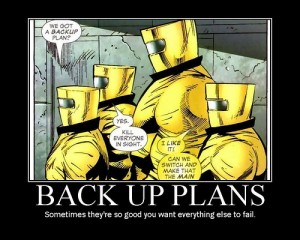
\includegraphics[width=\figwidth]{pics/9/47.png}
	\end{center}
\end{wrapfigure}
Instead of surprise or denial, all we got was confusion. 
The general stopped, looked at Sarge, then back to his group, then back to Sarge. 
He shrugged and was about to start speaking when Nubby spoke up and accused the other general of being Ourumov. 
When that didn't get a reaction Tink said the man in the cloak was obviously Ourumov and told him to take it off. 
The cloaked figure turned to the other general and asked the "Gue'vesa'o" what an Ourumov was. 
There was a brief discussion where it was explained that Ourumov was the name of the Lord General that commanded the eastern front on the south continent. 
Last they heard he was holed up on the far side of the moon, planning his revenge on the Inquisitor General.

So yeah, wrong bunch of traitors. 
Awkward...

Anyway, even if none of them was Ourumov, someone had recognized the name. 
Twitch was watching the Interrogator and Ivana for vampire ork shenanigans and noticed the valkyrie flinch like someone had tased her. 
He made several logical leaps, all of which were incorrect, but led him to the right response anyway. 
He screamed "PLAN B, PLAN B" and tackled the untouchable.

Plan B was like Plan A, except we were fighting everyone instead of just the Trader's men and the traitors. 
Sarge grabbed one if the supposedly friendly guards and threw him at one of the bodyguards while Nubby kicked the other in the groin with the full force of his augmetic legs. 
Doc and Tink used the split second of breathing room to dig out our weapons and Fumbles grabbed Twitch a roll of ductape.

Bane immediately drew his pistols and killed a bodyguard and the captain before he was forced to dodge a haymaker from Ivana. 
The haymaker completely missed the Interrogator and knocked out the traitor general that had been coming up behind him. 
Then cloaked figure and the surviving two officers started screaming about it being a trap, the bodyguard and guard Sarge had thrown shot each other, and the courtyard exploded into chaos.

\begin{wrapfigure}{O}{\figwidth}
	\begin{center}
		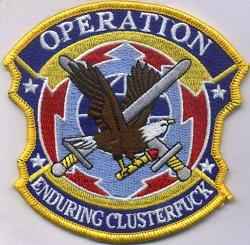
\includegraphics[width=\figwidth]{pics/9/48.png}
	\end{center}
\end{wrapfigure}
Honestly we didn't have any idea what was going on. 
Guards were killing other guards, reinforcements were coming in and trying to figure out who was the enemy, the traitors had scattered, and a very ominous sounding alarm was going off. 
The centerpiece of all this was a martial arts match between Bane and Ivana, which consisted entirely of him dodging her blows while asking her to "search her heart".

For our part we started throwing smokes in every direction as fast as we could dig them out and shot at anyone who seemed to be paying attention to us. 
Our goal was simple, we wanted to get onto that shuttle and get the hell out of there before we were all killed; 
the traitors and guards and traitor guards could kill each other to their hearts' content after we were gone. 
Sarge led us in a scrambling run from cover to cover as we wrestled with packs half full of dirt and flowers and the very unhappy untouchable.

Now that we knew to look for it, the Interrogator's screwed up probability field was obvious. 
Shots went wild, Doc and Nubby both jammed their guns, Twitch hit himself in the face with a rebounding smoke grenade, and Tink didn't even try to use his plasma gun. 
The techie and Fumbles kept their heads down and dragged the untouchable behind us as we ran.

\begin{wrapfigure}{O}{\figwidth}
	\begin{center}
		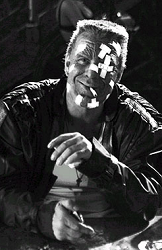
\includegraphics[width=\figwidth]{pics/9/49.png}
	\end{center}
\end{wrapfigure}
As bad as we were getting messed with by the Interrogator's field, the valkyrie and guards closer to Bane were getting it worse. 
Men would stumble into shots aimed at his back, guns would explode in their users hands, and one man threw the pin at him instead of the grenade, poor bastard. 
Ivana soaked a ton of punishment before a shotgun blast knocked her down to her knees, the Interrogator gave her a little bow and sprinted after us.

We made it to the shuttle without any major injuries, piled in, and gave the pilot a choice between an exciting new career in the Inquisition and a grisly death. 
Bane jumped in a second ahead of the slamming doors and we rose into the air as the villa began to explode below us. 
Several cars and fliers made it away before the whole thing went up and the infuriated voice hailed us over the vox. 
The Rogue Trader swore undying vengeance and promised Bane that he'd "get him next time", Sarge left the Interrogator to exchange witty banter and watched to make sure no one was following us.

When was finished tormenting the Trader Bane smiled his stupid grin and congratulated everyone on a job well done. 
We might all be rough around the edges and nowhere near as experienced as him, but we'd pulled through. 
In fact he'd be proud to have us as permanent members of his team, a few years learning from him would turn into real secret agents. 
Sarge smiled a grin even wider than the Interrogator's, signaled Twitch to turn off the Untouchable's limiter, and beat seven kinds of shit out of the smarmy bastard.

\begin{wrapfigure}{O}{\figwidth}
	\begin{center}
		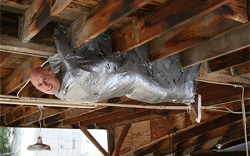
\includegraphics[width=\figwidth]{pics/9/50.png}
	\end{center}
\end{wrapfigure}
Tink's piloting skills were vastly improved by the Untouchable's aura of normality, he quickly familiarized himself with the shuttle's controls and the pilot was taped to a seat in the passenger area. 
While he flew and Sarge worked out his anger issues, Doc voxed the Rupert and updated him on the situation. 
The Inquisitor General looked like he'd been having a great time and was only moderately disappointed when we told him that Ourumov hadn't been there. 
He perked right back up when we told him about the traitors we had seen and gave him that tidbit about Ourumov hiding behind the moon.

The Rupert immediately dispatched several assault shuttles then gave us some every unwelcome orders, he wanted us to personally lead the assault and make sure Lord General Ourumov was captured alive. 
Well actually he gave the Interrogator that order, but Bane was taped to the untouchable and couldn't come to the vox right now. 
Anyhow it was an order and if we dithered about things for too long the Lord General would probably escape and the whole mission would be a wash. 
We raided what supplies we could from the shuttle, got into position near the moon and waited for our backup.

While we waited there was some discussion about what to do with the Interrogator, there was no way we were going to let him lead the assault. 
Nubby and Twitch were in favor of misplacing him, as in misplacing him out the airlock, but Sarge wasn't quite ready to kill a superior officer that hadn't actively tried to kill him. 
Doc suggestion of tranqing the Interrogator was gaining traction when Tink spoke up.

Perhaps, the techie suggested, we could use his abilities to help us. 
He was great in a fight if you weren't in the "danger zone" as he put it. 
So half an hour before our squad led the assault on the Lord General Ourumov Secret Moon Base, the Interrogator was shoved into the escape pod and fired at it like a boarding torpedo.

We left the tape on. 
Sarge said he'd probably be fine.

\begin{wrapfigure}{O}{\figwidth}
	\begin{center}
		\includegraphics[width=\figwidth]{pics/9/51.png}
	\end{center}
\end{wrapfigure}
So no shit, there we were, watching our Interrogator rocketing into the distance and preparing to assault the Secret Moon Base of a traitorous Lord General. 
That's not something you get to say often.

We swapped into one of the assault shuttles and borrowed some void gear for the assault, no sense dying of asphyxiation before we even got to the enemy. 
The plan was simple, kill or capture anyone who wasn't part of the strike force, the boys the Rupert sent us were pretty pumped to hear that we didn't have any crazy-complex strategies for them to follow. 
It was good that they were happy, because the assault began to look a lot more dangerous as we came around the moon. 


Lord General Ourumov's Secret Moon Base was not actually very secret, mostly because someone had parked a bright red Kroozer over it. 
Twitch alternated between ecstatically telling us that Orks really had been behind everyone and worrying about whether there were any Kommandos in the base.

As far as we could tell it wasn't attacking the base, just sort of hanging there. 
We were pretty sure that no one was dumb enough to try and hire a Freeboota as a transport, but it certainly looked like that was what was happening here. 
We put in a quick call to the Navy, then chilled our heels until a hail of macrocannon shots came in at an appreciable fraction of light speed. 
While the Orks re-evaluated their decision to hold still in what was mostly Imperial controlled space, we launched our assault.

Our bird was in the second wave, none of us had real experience in void battles, so it was better to wait for the fight to get inside before we participated. 
As battles go it was a pretty good one; 
we had more men, better troopers, and the element of surprise, it would have been a quick slaughter without the freebootas. 
The assault teams cut in from every direction, splitting up the defenders and wrecking the chain of command. 
They pinpointed the HQ within minutes and we moved in for the kill.

\begin{wrapfigure}{O}{\figwidth}
	\begin{center}
		\includegraphics[width=\figwidth]{pics/9/52.png}
	\end{center}
\end{wrapfigure}
This was the sort of fight we liked, the enemy was in front of us, our flanks were secure, and we were the only ones with a decent heavy weapon. 
There wasn't any screwing around with hallways and their limited cover, we just blasted through wall after wall, flashing the occupants then hitting the biggest hostile with an overcharged plasma shot. 
Tink didn't get many more kills than the rest of us, but almost every ork we bagged was all him and he only burned himself once. 
The real clincher was Fumbles though.

The psyker was doing wonderfully, a little praise and whatever Nubby had given him while Sarge and Doc weren't looking had really improved his morale. 
It's amazing how much it helps to have someone who can pinpoint hostiles on the other side of the wall for you and doubly amazing how much damage a simple invisible grenade can do. 
Fumbles didn't screw up a single time during the whole push and even managed to shoot someone with his laspistol, the little guy felt like a superhero and everyone within twenty or so meters felt like one too.

Of course battles didn't all go our way. 
Doc got to patch up all of us at some point or another and we saw at least a dozen assault troopers go down as we cut through the middle of their fights. 
Honestly we could have probably handled twice the number of hostiles we actually encountered, but none of us were complaining, we knew that our luck wouldn't hold out forever.

\begin{wrapfigure}{O}{\figwidth}
	\begin{center}
		\includegraphics[width=\figwidth]{pics/9/53.png}
	\end{center}
\end{wrapfigure}
Our push forward slowed and stalled as we neared the end, not because there was too much resistance, but because there wasn't any. 
The halls were empty except for corpses with autogun wounds. 
Sarge called a halt as we waited for our duct-taped untouchable to be brought forward by some troopers, we weren't going anywhere near the Interrogator without him.

Once the untouchable arrived we got him crammed into Sarge's pack like a toddler and made sure we could turn off his limiter in an instant. 
Our secret weapon ready, we carefully made our way forward until we heard voices and an ominous hum. 
Twitch edged around a doorway, flinched backwards, then waved us up. 
What we saw in there was at least the third weirdest thing any of us had encountered.

The Interrogator was tied to table and what looked like a ship's point-defense laser was suspended above him. 
A massive Ork with a gold plated cybork arm and a tricorn hat was slowly stomping in a circle around the table and a pair of gretchin were operating the laser's controls. 
As we watched a beam about the size of an arm crackled out and started rotating up the table towards Bane. 
The gouge it cut in the floor looked to be about ten meters deep.

While this was all rather odd, the outright weird part was what Bane and the Freeboota were doing. 
As the beam crawled towards the Interrogator's spread legs he didn't scream or plead, instead he calmly talked with the Ork.

\begin{wrapfigure}{O}{\figwidth}
	\begin{center}
		\includegraphics[width=\figwidth]{pics/9/54.png}
	\end{center}
\end{wrapfigure}
\greentext{>"You thot yous was more cunnin dan us, but Gol-Fingy's the cunninist Ork dere is, and I'M GOL-FINGY. Now dis here beamy deff lazer is powful enuf to poject a spot on da moon. But not dis moon, like if dere were anuver one behind it dere'd be a spot on it."}


"Foul Xenos, do you expect me to talk?"

\greentext{>"Wot? Na you daft git, I spect you to die!"}


"...It's not moving very fast."

\greentext{>"Shaddup."}


"While we're waiting why don't you tell me about your evil plans? 
It's not like I'm going to escape to tell anyone."

\greentext{>"Uhhhh don really got one of dose. Was gonna take da posh umies money den push 'im out the airlock, but since my Kroozer's run off I'm really jus plannin to cut some nosy 'ummie in 'alf wif my deff laser."}


"Oh… I don't suppose you'd be willing to let me go? 
Or have a beautiful and emotionally vulnerable henchwoman?"

\greentext{>"Can't you grots make dis fing go any fasta?"}


\begin{wrapfigure}{O}{\figwidth}
	\begin{center}
		\includegraphics[width=\figwidth]{pics/9/55.png}
	\end{center}
\end{wrapfigure}
At this point the beam was getting pretty close and we felt it was time to do something. 
We weren't quite ready just to let the Interrogator die, not when the mission was almost over and we knew we could subdue him at a moments notice. 
Tink linked up a shot on what looked like the most critical component of the laser, the rest of us got ready to open fire, and Fumbles sat in the corner since we wouldn't let him use his powers this close to the Interrogator.

Twitch fired, the gretchins both exploded, and the laser went haywire. 
Before it cut off completely the beam somehow split apart and simultaneously cut every single one of the Interrogator's restrains, this did not surprise any of us. 
The first volley of las fire hit the Freeboota square in the chest, the second was stopped by his augmetic arm, and the third was delayed as we scattered away from a well thrown stikkbomb. 
Sarge and Doc took the right, peppering him with unaimed las-fire while frantically dodging a rain of slugs. 
On the other side Twitch, Nubby, and Tink all took careful aim at the back of the Ork's head.

Twitch's gun jammed, Nubby managed to hit the floor AND the ceiling, and Tink's plasma gun overheated. 
All three troopers stared at each other in panic, then scattered as another stikkbomb landed between them. 
As they ran they were treated to the sight of Bane rising up behind the Ork with a comically small switchblade. 
The way he jammed it into the Freeboota's ear wasn't funny though.

\begin{wrapfigure}{O}{\figwidth}
	\begin{center}
		\includegraphics[width=\figwidth]{pics/9/56.png}
	\end{center}
\end{wrapfigure}
The massive Ork started flailing around, frantically trying to dislodge the Interrogator. 
Everyone took a second to appreciate the sight, then opened up on full auto, only pausing to reload or clear jams. 
As a side note, none of us bothered to try and miss Bane, we figured he'd take care of that himself.

The Freeboota finally dislodged the Interrogator and threw him into a bank of cogitators, but he was obviously on his last legs. 
A final few volleys reduced him to a bleeding pile of meat, and a detpack made sure he wasn't getting back up. 
Twitch used three detonators for that and we still had to set it off by shooting it with a lasgun from the hallway. 
That done, there was a round of high-fives and celebratory smokes, which were interrupted by the sound of approaching boots.

We all dove into cover, but Bane just stood there and faced down the dozen storm troopers than thundered through the far door. 
Behind them came a man in a Lord General's uniform and Ivana in a suit of power armor. 
There was a brief, surprised staring match then Lord General Ourumov started monologuing.

\begin{wrapfigure}{O}{\figwidth}
	\begin{center}
		\includegraphics[width=\figwidth]{pics/9/57.png}
	\end{center}
\end{wrapfigure}
It wasn't the best monologue, we'd heard one or two really good ones, and this was only sort of middling. 
Sarge signalled everyone to start lining up their shots, quietly calling targets over the comm while the idiots bantered.

It was an agonizing wait, Nubby and Tink both nearly cracked before it was over, but it paid off. 
Bane dismissed something the traitor said, turned to face Ivana and asked her if she would listen to her boss… or her heart? 
Doc threw up a little in his mouth.

The valkyrie went from zero to sixty in about half a second, the two storm troopers nearest to her were reduced to chunky salsa. 
Bane did some sort of ridiculous backflip behind a table, hefted the freeboota's shoota and somehow managed to use it to hose fire across the troopers. 
While they did the showy stuff, we placed four solid headshots and knocked out the door controls behind the traitor.

The fight ended with Ourumov being suspended from one of Ivana's fists while she used the other lift the Interrogator high enough for a sloppy makeout. 
Sarge voxed the Rupert to report our success while Tink and Doc pried the terrified Lord General down and tranqued him. 
Nubby and Twitch retrieved Fumbles and verified that no hostiles were left in the area. 
At this point Sarge called the mission a success, and started to reach behind his back to turn off the Untouchable's limiter. 
A second later he was covered with a spray of bone and meat as Bane casually blew the taped-up prisoner's head off.

Couldn't let a traitor like that live, could he?

\begin{wrapfigure}{O}{\figwidth}
	\begin{center}
		\includegraphics[width=\figwidth]{pics/9/58.png}
	\end{center}
\end{wrapfigure}
We were all on pins and needles, it was like being trapped in a very small room with a sleeping ursid. 
Doc carefully pulled the Lord General back, Tink swapped his plasma gun for a las-pistol, Twitch pushed Fumbles back, and Nubby made sure he had a clear path to the door. 
Sarge quietly asked the Interrogator what he was going to do now. 
Bane looked at each of us in turn, then to Ivana, then back to Sarge. 
An expression that closely resembled thought crossed his face. 
Then it vanished to be replaced with his vapid smile, "Now" he bellowed "we PARTY!".

Everyone breathed a sigh of relief and Sarge facepalmed.

The shit you put up with in this job…

Anyway we followed him out, it was easier than fighting it. 
We got back on a shuttle and flew back down to the Rupert's mansion where the Interrogator instigated a night of wild hedonism the likes of which none of us had ever seen. 
And we didn't see it now either, we locked ourselves in our rooms and tried to figure out just what the hell we were going to do now.

Tink and Twitch voted for finding another untouchable and ending this shit now. 
The man was obviously a complete psychotic, with no sense of right, wrong, or reality. 
Sarge and Doc weren't so sure though, if he saw us coming shit would go down real fast, and was still technically murdering a superior officer. 
The Inquisition frowned on that sort of thing. 
Nubby advised patience, we'd managed to hide from a shitty Interrogator before, we could do it again.

Fumbles suggested we ask the people standing in the hallway about a second before they knocked.

\begin{wrapfigure}{O}{\figwidth}
	\begin{center}
		\includegraphics[width=\figwidth]{pics/9/59.png}
	\end{center}
\end{wrapfigure}
Three men entered our room, we recognized the one on the right. 
He was the Interrogator who'd been our nominal superior while we were playing teacher, now he was all done up in combat gear. 
The man on the left was an untouchable, but not a normal one, he had an aura like Fumbles in a suicidal depression, and that was with his limiter on. 
The middle man was tall, covered with scars and augmetics, and had a servo skull hovering over his shoulder.

They made themselves comfortable, greeted us all by name, then congratulated us on surviving our mission. 
We kept our mouths shut and waited for the shoe to drop. 
Eventually they got tired of playing the big scary Inquisitors and only getting monosyllabic responses, the middle one stood back up and fished around in his shirt for something. 
He drew out a rosette which identified him as a member of the Ordos Hereticus and asked what our opinion was of Interrogator Bane Johns.

Sarge sat up a bit straighter and asked why he was so interested in the opinion of a bunch of grunts. 
The Inquisitor smiled back and said we were the first team to survive a mission with him, so were the best men to judge whether he was a dangerous untrained psyker who might become a serious threat to the Imperium. 
Every single one of us grinned like a kid in a candy store. 


Unfortunately the moment was slightly spoiled by Twitch saying that we thought Bane was a vampire ork.

\begin{wrapfigure}{O}{\figwidth}
	\begin{center}
		\includegraphics[width=\figwidth]{pics/9/60.png}
	\end{center}
\end{wrapfigure}
They let us watch when they stormed into party, deactivated the limiter, and dragged the drunken Interrogator out behind them. 
It was glorious, especially when he kept trying to do martial-arts moves and hit himself. 
It must suck to live a life where everything you do just magically works, then have it taken away. 
Nubby suggested that we should send him a card or something, perhaps a tasteful goodbye message like "Enjoy your life in a psi-shield inquisitorial dungeon, don't forget to write". 
We really shouldn't have laughed at that, it only encouraged him.

When they took Bane Ivana had tried to put up a fight, but Oak's personal Interrogator drew some sort of small sleek pistol and the valkyrie was asleep before she got half a meter. 
We heard him tell his men to pack her up, he knew someone who might want to offer her job. 
We decided that was as fair a chance as any of us had gotten, and went to bed.

We stuck around the planet for a few days after the Inquisitor left, partially to see if the Rupert needed help, but mostly because we had to wait for a ship that was going our way. 
The dapper man was a little concerned over what had happened to our Interrogator, but accepted our assurance that it was all for the best. 
He would've loved to spend some time swapping tales with us, unfortunately he was rather busy running the war. 
The Rupert said he'd intended to hand off command to some of the less corrupt generals after the purges, but everyone seemed to think he was doing an wonderful job and wanted him to stay until the war ended.

Hopefully that wouldn't take too many years, morale had improved greatly after the purge, and deserters no longer seemed to be disappearing off planet in surprisingly large numbers. 
He put that down to the execution of Ourumov and all of his contacts, but we remembered the other group of traitors and weren't so sure.

\begin{wrapfigure}{O}{\figwidth}
	\begin{center}
		\includegraphics[width=\figwidth]{pics/9/61.png}
	\end{center}
\end{wrapfigure}
A few weeks later we disembarked onto Oak's ship to find a runner waiting for us. 
Doc had thought ahead, he and Sarge had put together a full report during our travel time, so instead of a grueling oral examination we just handed over the dataslate and went our way.

The welcome back party was much more our speed, less loud music and mindless extravagance, more old friends. 
Nubby captivated everyone with the completely true tale of our adventure and his heroic exploits, Doc disappeared with his lady friend, Twitch introduced Fumbles to some new friends, and Tink managed to talk to Hannah the cog-girl without getting slapped. 
Sarge watched it all and felt proud, then ducked out early after a runner passed him a note.

The argument in Oak's office was heard by no one and no device recorded it. 
If someone had been there to hear it though, they might have heard the phases "killed over thirty teams" and "you used us like guinea pigs" repeated a few times. 
They might also have heard an older, quieter voice explaining that only one type of person is allowed to dictate team composition on his ship.

A few hours later Interrogator Greg Sargent left Oak's office and returned to the party holding a dataslate. 
He sat, played with it for a while, then walked over to where Nubby and Twitch were sitting and swapping stories with old friends. 
He took a seat, grabbed a drink, and in rhetorical way asked:

\greentext{>Where the hell is Tau Space?}

